%  ========================================================================
%  Copyright (c) 1985 The University of Washington
%
%  Licensed under the Apache License, Version 2.0 (the "License");
%  you may not use this file except in compliance with the License.
%  You may obtain a copy of the License at
%
%      http://www.apache.org/licenses/LICENSE-2.0
%
%  Unless required by applicable law or agreed to in writing, software
%  distributed under the License is distributed on an "AS IS" BASIS,
%  WITHOUT WARRANTIES OR CONDITIONS OF ANY KIND, either express or implied.
%  See the License for the specific language governing permissions and
%  limitations under the License.
%  ========================================================================
%

% Documentation for University of Washington thesis LaTeX document class
% by Jim Fox
% fox@washington.edu
%
%    Revised 2020/02/24, added \caption()[]{} option.  No ToC.
%
%    Revised for version 2015/03/03 of uwthesis.cls
%    Revised, 2016/11/22, for cleanup of sample copyright and title pages
%
%    This document is contained in a single file ONLY because
%    I wanted to be able to distribute it easily.  A real thesis ought
%    to be contained on many files (e.g., one for each chapter, at least).
%
%    To help you identify the files and sections in this large file
%    I use the string '==========' to identify new files.
%
%    To help you ignore the unusual things I do with this sample document
%    I try to use the notation
%       
%    % --- sample stuff only -----
%    special stuff for my document, but you don't need it in your thesis
%    % --- end-of-sample-stuff ---


%    Printed in twoside style now that that's allowed
%
 
\documentclass [11pt, proquest] {uwthesis}[2020/02/24]
 
%
% The following line would print the thesis in a postscript font 

% \usepackage{natbib}
% \def\bibpreamble{\protect\addcontentsline{toc}{chapter}{Bibliography}}

\setcounter{tocdepth}{1}  % Print the chapter and sections to the toc

\usepackage{amsmath}
\usepackage{amssymb}
\usepackage{xspace}
\usepackage{natbib}
\usepackage{csvsimple}
\usepackage{microtype}
\usepackage{tikz}
\usepackage{tikz-qtree}
\usepackage{tabularx}
\usepackage{makecell}
\usepackage{algorithm2e}
\usepackage{hhline}
\usetikzlibrary{hobby,arrows,backgrounds,calc,trees,automata}


\pgfdeclarelayer{background}
\pgfsetlayers{background,main}

\newcommand{\convexpath}[2]{
[   
    create hullnodes/.code={
        \global\edef\namelist{#1}
        \foreach [count=\counter] \nodename in \namelist {
            \global\edef\numberofnodes{\counter}
            \node at (\nodename) [draw=none,name=hullnode\counter] {};
        }
        \node at (hullnode\numberofnodes) [name=hullnode0,draw=none] {};
        \pgfmathtruncatemacro\lastnumber{\numberofnodes+1}
        \node at (hullnode1) [name=hullnode\lastnumber,draw=none] {};
    },
    create hullnodes
]
($(hullnode1)!#2!-90:(hullnode0)$)
\foreach [
    evaluate=\currentnode as \previousnode using \currentnode-1,
    evaluate=\currentnode as \nextnode using \currentnode+1
    ] \currentnode in {1,...,\numberofnodes} {
  let
    \p1 = ($(hullnode\currentnode)!#2!-90:(hullnode\previousnode)$),
    \p2 = ($(hullnode\currentnode)!#2!90:(hullnode\nextnode)$),
    \p3 = ($(\p1) - (hullnode\currentnode)$),
    \n1 = {atan2(\y3,\x3)},
    \p4 = ($(\p2) - (hullnode\currentnode)$),
    \n2 = {atan2(\y4,\x4)},
    \n{delta} = {-Mod(\n1-\n2,360)}
  in 
    {-- (\p1) arc[start angle=\n1, delta angle=\n{delta}, radius=#2] -- (\p2)}
}
-- cycle
}
\tikzset{
  leaf/.style={sibling distance=5mm}
}

% ==========   Local defs and mods
\definecolor{uwpurple}{RGB}{128,0,128}
\definecolor{darkgreen}{RGB}{0,64,0}
\newcommand{\jln}[1]{\textcolor{uwpurple}{\textit{[{#1} --JLN]}}}
\newcommand{\sak}[1]{\textcolor{olive}{\textit{[{#1} --SK]}}}
\newcommand{\aba}[1]{\textcolor{darkgreen}{\textit{[{#1} --AA]}}}
\newcommand{\rb}[1]{\textcolor{blue}{\textit{[{#1} --RB]}}}

\newcommand{\modified}[1]{\textcolor{black}{{#1}}}
\newcommand{\modifiedagain}[1]{\textcolor{black}{{#1}}}

\newcommand{\hmax}[0]{\texttt{max}}
\newcommand{\hmin}[0]{\texttt{min}}
%\newcommand{\rewrites}[0]{\mathop{\rightarrow}\limits_{\scriptscriptstyle{R}}}
\newcommand{\rewrites}[0]{\:\rightarrow_{R}\:}
%\newcommand{\rewrites}[0]{\longrightarrow}
%\newcommand{\rewrites}[0]{\rightharpoonup}
\newcommand{\pred}[0]{\textrm{ if }}
\newcommand{\hfalse}[0]{\texttt{false}}
\newcommand{\htrue}[0]{\texttt{true}}
\newcommand{\hsel}[0]{\texttt{select}}
\usepackage{syntax}

%% Macros for quantities
\newcommand{\NumApps}{{\color{black} 10}\xspace}
\newcommand{\NumRulesFixed}{{\color{black} 4}\xspace}
\newcommand{\NumPredicatesRelaxed}{{\color{black} 17}\xspace}
\newcommand{\NumOrderingProblems}{{\color{black} 8}\xspace}
\newcommand{\NumRulesSynthesized}{{\color{black} 4127}\xspace}
\newcommand{\NumOpSequences}{{\color{black} 6246}\xspace}
\newcommand{\NumFailureExamples}{{\color{black} 61000}\xspace}
\newcommand{\NumSimplifiedExpressions}{{\color{black} 195371}\xspace} 
\newcommand{\NumBugsAutomated}{{\color{black} 5}\xspace}
\newcommand{\NumOriginalRules}{{\color{black} 999}\xspace}
\newcommand{\NumZdivCoqProvedRules}{{\color{black} 141}\xspace}
\newcommand{\NumZdivFalseRules}{{\color{black} 44}\xspace}
\newcommand{\NumZdivRelaxedPredicates}{{\color{black} 37}\xspace}

\newtheorem{theorem}{Theorem}[section]

% --- sample stuff only -----
% These format the sample code in this document

\usepackage{alltt}  % 
\newenvironment{demo}
  {\begin{alltt}\leftskip3em
     \def\\{\ttfamily\char`\\}%
     \def\{{\ttfamily\char`\{}%
     \def\}{\ttfamily\char`\}}}
  {\end{alltt}}
 
% metafont font.  If logo not available, use the second form
%
% \font\mffont=logosl10 scaled\magstep1
\let\mffont=\sf
% --- end-of-sample-stuff ---
 
\usepackage{hyperref}


\begin{document}
 
% ==========   Preliminary pages
%
% ( revised 2012 for electronic submission )
%

\prelimpages
 
%
% ----- copyright and title pages
%
\Title{a dissertation}
\Author{Julie L. Newcomb}
\Year{2021}
\Program{Computer Science and Engineering}

\Chair{Name of Chairperson}{Title of Chair}{Department of Chair}
\Signature{First committee member}
\Signature{Next committee member}
\Signature{etc}

\copyrightpage

\titlepage  

 
%
% ----- signature and quoteslip are gone
%

%
% ----- abstract
%


\setcounter{page}{-1}
\abstract{%
This sample dissertation is an aid to students who are attempting
to format their theses with \LaTeX, a sophisticated
text formatter widely used by mathematicians and scientists everywhere.
 
\begin{itemize}
\item It describes the use of a specialized
macro package developed specifically for thesis production
at the University.
The macros customize \LaTeX\ for the correct thesis style,
allowing the student to concentrate on the substance of
his or her text.%
\footnote{See Appendix A to obtain the source to this
 thesis and the class file.}
\item It demonstrates the solutions to a variety of
formatting challenges found in thesis production.
\item It serves as a template for a real dissertation.
\end{itemize}
}
 
%
% ----- contents & etc.
%
\tableofcontents
\listoffigures
%\listoftables  % I have no tables
 
%

 
%
% ----- acknowledgments
%
\acknowledgments{% \vskip2pc
  % {\narrower\noindent
  The author wishes to express sincere appreciation to
  University of Washington, where he has had the opportunity
  to work with the \TeX\ formatting system,
  and to the author of \TeX, Donald Knuth, {\it il miglior fabbro}.
  % \par}
}

%
% ----- dedication
%
\dedication{\begin{center}to my dear wife, Joanna\end{center}}

%
% end of the preliminary pages
 
 
 
%
% ==========      Text pages
%

\textpages

% ========== chapters
\chapter{Introduction}
\label{sec:intro}

this is the introduction.

this is a change made in overleaf.
\chapter{Background}
\label{chapter:overview}

We define term rewriting systems and give some background. We then discuss the use of term rewriting systems in the Halide compiler and describe the two main such systems, the \emph{simplifier} and the \emph{variable solver}. We describe the rewriting algorithm used by the Halide compiler and discuss the requirements that led to its design choices. 

The Halide compiler contains term rewriting systems operating over the space of Halide expressions (see appendex~\ref{a:grammar} for
the full Halide expression grammar). The language of Halide expressions
operates over vectors and scalars of integers, booleans, and real values.  However, in
this work we concentrate on the TRS as it applies to integer and boolean values, for
both vectors and scalars, because the most important uses of the TRS within the compiler
apply to these types.  In this section, we give some background on term rewriting systems.
We then describe how the Halide compiler uses term rewriting systems as reasoning engines
and the design decisions that motivate the custom rewriting engine, as well as the scope
of our work.

\section{Term Rewriting Systems}

Term rewriting systems~\citep{gorn1967} are sets of \textit{rewrite rules} used to transform expressions into a new form.  Such systems are widely
used in theorem proving~\citep{baader1999term} and abstract interpretation~\citep{cousot1977abstract, cousot1979systematic}.

Terms are defined inductively over a set of variables $V$ and a set of function symbols $\Sigma$. Every variable $v \in V$ is a term, and for any function symbol $f \in \Sigma$ with arity $n$ and any terms $t_1, ..., t_n$, the application of the symbol to the terms $f(t_1, ..., t_n)$ is also a term. (Constants are considered zero-arity functions.) We refer to the set of terms constructed from the variables $V$ and the function symbols $\Sigma$ as $T(\Sigma, V)$.

A \emph{rewrite rule} is a directed binary relation $l \rewrites r$ such that $l$ is not a variable, and all variables present in $r$ are also present in $l$ (i.e., $\mathcal{V}ar(l) \supseteq \mathcal{V}ar(r)$). A set of rewrite rules is called a \emph{term rewriting system}.

Consider a set of terms $T(\Sigma, V)$ such that $\Sigma = \{\clubsuit, \diamondsuit\}$ and $V$ is an infinite set of variables. Let the term rewriting system $R$ consist of a single rule:

\[ R = \{ x_1 \clubsuit x_2 \rewrites x_1 \diamondsuit x_2 \} \]
We use $R$ to rewrite the term

\[ 
(y_1 \diamondsuit y_1) \clubsuit (y_2 \clubsuit y_3)
\]
The first step is matching; we find a substitution that will unify the left-hand side (LHS) of the rule with the term we are rewriting. Here, one possible substitution is:

\[
\{ x_1 \mapsto (y_1 \diamondsuit y_1), x_2 \mapsto (y_2 \clubsuit y_3) \}
\]
We then apply this substitution to the right-hand side (RHS) of the rule to obtain the rewritten version of the original term:

\[ 
(y_1 \diamondsuit y_1) \diamondsuit (y_2 \clubsuit y_3)
\]


\section{Term rewriting systems in the Halide compiler}



%\subsubsection{TrimNoOps}
%
%When compiling a pipeline, the Halide compiler will attempt to truncate loop bounds to the regions where work is actually performed. The TrimNoOps %phase examines a for loop and attempts to prove that some regions of the loop are no-ops; if it can show this, it rewrites the loop so those %regions are never visited. The variable solver used in performing this reasoning.
%
%For example, consider a for loop that applies the following function over some range of $x$ and $y$:
%
%\begin{verbatim}
%f(x, y) = x + y + select((x == 10) && (x < y), 1, 0)
%\end{verbatim}
%
%After several compilation phases, the for loop is transformed into:
%
%\begin{verbatim}
%f = {
%	for(y, y_min, y_extent) {
%		for(x, x_min, x_extent) {
%			f[(y * stride + x) - (y_min * stride + x_min)] = x + y
%		}
%	}
%	for(y, y_min, y_extent) {
%		for(x, x_min, x_extent) {
%			f[(y * stride + x) - (y_min * stride + x_min)] = 
%			f[(y * stride + x) - (y_min * stride + x_min)] + select((x == 10) && (x < y), 1, 0)
%		}
%	}
%}
%\end{verbatim}

%%% the example itself is easy to understand but it doesn't actually make use of the variable solver in solving it (it does call it, just doesn't get back interesting results)

\begin{figure*}
\begin{tabular}{cccc}

%\Tree [.+ [.- [.min a b ] [.max c c ] ] [.max c c ]]
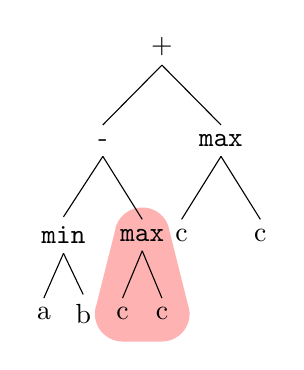
\begin{tikzpicture}[level distance=12mm]
\tikzstyle{level 1}=[sibling distance=15mm]
\tikzstyle{level 2}=[sibling distance=10mm]
\tikzstyle{level 3}=[level distance=10mm,sibling distance=5mm]


%\Tree [.+ [.- [.min a b ] c ] [.max c c ]]
\node (+) {+}
  child { node (-) {-}
    child { node (min) {\hmin}
      child {node (a) {a}}
      child {node (b) {b}}
    }
    child { node (max2) {\hmax}
      child {node (c4) {c}}
      child {node (c5) {c}}
    }
  }
  child { node (max) {\hmax}
    child { node (c2) {c}}
    child { node (c3) {c}}
  };
\begin{pgfonlayer}{background}
\fill[red,opacity=0.3] \convexpath{c4,max2,c5}{10pt};
\end{pgfonlayer}
\end{tikzpicture}

&
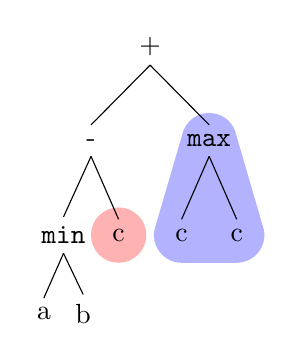
\begin{tikzpicture}[level distance=12mm]
\tikzstyle{level 1}=[sibling distance=15mm]
\tikzstyle{level 2}=[sibling distance=7mm]
\tikzstyle{level 3}=[level distance=10mm,sibling distance=5mm]
%\Tree [.+ [.- [.min a b ] c ] [.max c c ]]
\node (+) {+}
  child {  node (-) {-}
    child { node (min) {\hmin}
      child {node (a) {a}}
      child {node (b) {b}}
    }
    child { node (c) {c}}
  }
  child { node (max) {\hmax}
    child { node (c2) {c}}
    child { node (c3) {c}}
  };
\begin{pgfonlayer}{background}

\fill[blue,opacity=0.3] \convexpath{c2,max,c3}{10pt};
%\fill[red,opacity=0.3] \convexpath{c}{10pt};
\draw[fill=red,opacity=0.3,draw=none](c) circle (10pt);

\end{pgfonlayer}
\end{tikzpicture}
&
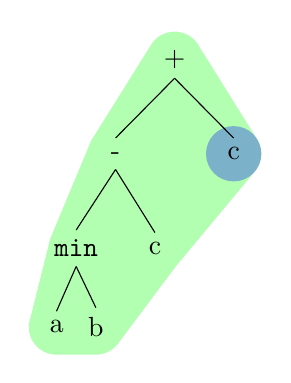
\begin{tikzpicture}[level distance=12mm]
\tikzstyle{level 1}=[sibling distance=15mm]
\tikzstyle{level 2}=[sibling distance=10mm]
\tikzstyle{level 3}=[level distance=10mm,sibling distance=5mm]
%\Tree [.+ [.- [.min a b ] c ] c ]
\node (+) {+}
  child { node (-) {-}
    child { node (min) {\hmin}
      child {node (a) {a}}
      child {node (b) {b}}
    }
    child { node (c) {c} }
  }
  child { node (c2) {c}};



  \begin{pgfonlayer}{background}
\fill[green,opacity=0.3] \convexpath{b,a,min,-,+,c2,c}{10pt};
\draw[fill=blue,opacity=0.3,draw=none](c2) circle (10pt);
%\draw[red,fill=blue,opacity=0.3](c2.north) to[closed,curve through={($(c2.north east)!1.0!(c2.south east)$) .. ($(c2.south west)!1.0!(c2.north west)$)}] (c2.north);
\end{pgfonlayer}
\end{tikzpicture}
&
\vspace{0pt}
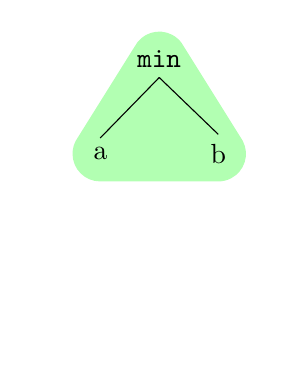
\begin{tikzpicture}[level distance=12mm]
\tikzstyle{level 1}=[sibling distance=15mm]
\tikzstyle{level 2}=[sibling distance=10mm]
\tikzstyle{level 3}=[level distance=10mm,sibling distance=5mm]
\node (min) {\hmin}
  child { node (a) {a}
     % [red,opacity=0.0]
    child {     [red,opacity=0.0] node (fake1) {f}
      child {    [red,opacity=0.0] node (fake2) {f}}
      child {    [red,opacity=0.0] node (fake3) {f}}
    }
    child {     [red,opacity=0.0] node (fake4) {f}
    [red,opacity=0.0]
    child { [red,opacity=0.0] node (fake) {f}}
    child { [red,opacity=0.0] node (fake2) {f}}
    }
  }
  child { node (b) {b}
     % [red,opacity=0.0]
    child {     [red,opacity=0.0] node (fake5) {f}}
    child {     [red,opacity=0.0] node (fake6) {f}}
  };
  \begin{pgfonlayer}{background}
\fill[green,opacity=0.3] \convexpath{a,min,b}{10pt};
\end{pgfonlayer}

\end{tikzpicture} \\
(i) & (ii) & (iii) & (iv)
\end{tabular}
\caption{We demonstrate the Halide rewriting algorithm using a TRS $R = \{\hmax(x, x) \rewrites x, (x - y) + y \rewrites x\}$ and an expression $\hmin(a,b) - \hmax(c,c) + \hmax(c,c)$. The algorithm attempts to simplify all subtrees bottom up; here, no rule applies to $\hmin(a,b)$ so it is not changed. Next (i), rule 1 rewrites $\hmax(c,c)$ to $c$. No rule applies to $\hmin(a,b) - c$, so we move to the rightmost subtree and rewrite again (ii) to obtain $c$ from $\hmax(c,c)$. Finally, we consider the entire tree $\hmin(a,b) - c) + c$ (iii) and apply rule 2 to produce $\hmin(a,b)$. No rules match this expression, so we are left with $\hmin(a,b)$ (iv).}
\label{fig:algoexample}
\end{figure*}

\subsection{The Halide rewriting algorithm}
\label{sec:customalgo}

In a term rewriting system, a single rule may be able to match an input expression in 
multiple ways, and there may be multiple rules in the ruleset which could be used 
to rewrite the expression. A term rewriting algorithm might choose one of many alternatives 
and later backtrack if it turns out not to be fruitful; it might make use of 
heuristics to choose a next step; it might exercise all the alternatives and keep 
the results in equivalence classes, as in an e-graph. The Halide term rewriting algorithm
keeps only one expression in state and applies rules greedily, in a fixed priority.
This is very fast and requires very little memory; the tradeoff is that the algorithm 
may pick the ``wrong'' rule and have no way of undoing that decision. 
Since the rewriter is invoked thousands of times with each call of the compiler, 
it chooses to sacrifice some solving power in exchange for performance.

The Halide term rewriting algorithm simplifies an input expression in a
depth-first, bottom-up traversal of the expression DAG. At each node, it 
uses the root node to pick a list of rules, then
attempts to match the subtree expression with the rule LHSs in a fixed priority. Matching
is performed purely syntactically, using C++ template metaprogramming.
 Halide rewrite rules contain special metavariables,
called \emph{symbolic constants}, that can match only with constant values; all other
variables can match any subterm as usual.
When a match is found, the algorithm rewrites the
subtree expression using the RHS of that rule, and then attempts to simplify the
subtree expression again. If no rule matches the subtree, the traversal
continues; when the entire expression cannot be simplified further, the
rewritten expression is returned. See Figure~\ref{fig:algoexample} for a worked
example.

The rewrite rules optionally contain a compile-time predicate guard. 
These guards contain only symbolic constants\footnote{Existing 
rules sometimes have predicates that check if
  non-constant variables can be shown to have certain properties at compile
  time, but these are expensive and used sparingly.}; when the LHS of a rule
matches an expression, its guard is evaluated and only if it
is true will the rewrite be applied.

Halide rewrite rules are applied in a fixed priority, organized so that the TRS 
first attempts very basic rules such as constant folding, then tries more specific 
rules before more general ones. (We do not evaluate the current rule priority in this work.)

Associativity and commutativity laws are particularly troublesome for term rewriting systems. 
For one expression $e$, the number of semantically equivalent expressions grows 
exponentially in terms of the number of AC operations $e$ contains. Some term rewriting 
systems perform a full \emph{AC matching} step during rewriting. Halide's TRS does not
perform this matching, but instead
includes multiple AC variations of rules.
However, a small number of Halide's rewrite rules have the effect of canonicalizing some commutative
expressions. (For example, if a commutative expression has a multiplication as its 
first operand and a subtraction as its second operand, a rule will switch their positions.)
These rules are all early in the application priority, so later rules can rely on
expressions having a quasi-canonical form.

\subsubsection{Why Not Z3?}
\begin{table}
\caption{We compare the performance of Z3 and the Halide TRS in proving a set of 4304 expressions gathered from realistic compiler output. Note that expressions in the ``not proven'' column include expressions that are true but not found to be so by the solvers as well as expressions that are not true. }
\centering
\begin{tabular}{l|r|r|r}
Tool & Runtime & Proven expressions & Not proven \\
\hline
Z3 & 7m29s & 1125 & 3179 \\
Halide TRS & 2s & 885 & 3419 
\end{tabular}
\label{tab:simplifiervsz3}
\end{table}


Given that we make use of the Z3 solver~\citep{de2008z3} for both verification and synthesis, it is natural to ask why Halide could not simply call Z3 for simplification. Z3 is the product of extensive development and is a very powerful, general-purpose solver. However, the Halide term rewriting system has a few key properties that Z3 does not: deterministic output, low memory and compute requirements, and domain-specific optimizations.

As discussed above, the Halide compiler must return the same schedule every time the same pipeline is run. Z3 can fix a random seed, but long-running queries may complete on a more powerful server while timing out on a different machine.

While the Halide algorithm is less powerful than Z3, its deterministic, greedy rule application strategy
gives it a smooth performance curve, whether it succeeds or fails in simplifying an input expression.
A solver like Z3 tends to give very good performance most of the time but gets bogged down in difficult cases, requiring the use of timeouts. The Halide algorithm ``fails fast'': on an input expression which does not match any rule,  the Halide algorithm will complete in time linear to the size of the expression, taking on the order of one CPU cycle per term in the expression per rule in the TRS. To demonstrate this performance tradeoff, we gathered 4304 expressions from queries the Halide compiler made when compiling realistic pipelines, including provably true expressions and expressions that are not provably true. Z3 could prove more expressions true (within a 60 second timeout), but was starkly less performant. As shown in Table~\ref{tab:simplifiervsz3}, Z3 took over 7 minutes to check the set of expressions while the Halide TRS took just 2 seconds. This set of expressions is much smaller than the number of calls the compiler makes to the rewriter in compiling a single pipeline.

Because the Halide algorithm at every step chooses one rule to apply to the single expression it is working on, it scales well in terms of the number of rules in the TRS. See Section~\ref{ssec:compilationspeed} for an evaluation of the effects of adding newly synthesized rules on the performance of the compiler. 

Finally, although Z3 can simplify expressions, simply reducing the size of an expression is not necessarily the goal for the compiler. For example, gathering like terms in some cases can actually prevent Halide or LLVM optimizations from applying. The Halide rewriter uses a domain-specific strategy to guide expressions into more optimizable forms and can be changed or tuned as needed if further optimizations are discovered. 

\subsection{Completeness of the Halide TRS}
\label{sec:completion}

We know by observation that the Halide simplifier TRS cannot prove certain equalities 
that are in fact true, or reduce certain expressions that can be further simplified. 
Our goal is to learn new rules that would strengthen the TRS and allow it to make
further progress on these ``stuck'' expressions. This goal seems similar to that of 
\emph{completion}, which constructs a decision procedure through syntatic rewrites
for a set of identities. We do not use completion directly, although
our synthesis algorithm could be considered analogous to completion in some ways.

In the standard Knuth-Bendix completion algorithm~\citep{knuth1983simple}, we take a
finite set of identities $E$ and a reduction order $>$ on terms as inputs; if successful, the
algorithm will return a finite, convergent set of rules $R$ that is equivalent to 
$E$. The algorithm may also fail, or fail to terminate. At each step the algorithm
maintains a set of identities and a set of rules, both of which can be updated; the 
algorithm may transform an identity into a new rule, find a new identity as a 
consequence of the ruleset, or use the present ruleset to refine either an identity 
or a rule. The algorithm runs until the ruleset has converged; specific implementations
may use some conditions under which to terminate with a failure.

No finite set of identities exists for the theory of integers. We could
fix a set of identities to use in a completion procedure, but choosing these axioms
is a non-trivial task. One issue is that the theory contains axioms such as commutativity;
an identity such as $x + y \equiv y + x$ cannot be oriented by any possible reduction 
order, so our completion algorithm cannot make use of this fact. Another is that any
sufficiently powerful set of identities would almost certainly result in a non-terminating
completion procedure.  In addition, even if we use a subset of the Halide TRS for our
identities (thus yielding a confluent Halide TRS), our experience shows that many
failures in the compiler's use of the TRS are due to missing semantic facts that are not
derivable from the current Halide ruleset.

%%% SAK: I integrated this into a sentence above.  Not sure we need this much text.
%% \modified{One approach might be to transform the existing Halide TRS into a set of undirected
%% identities $E_R$ and use it together with a reduction order as inputs to a completion procedure. 
%% If successful, this would yield a confluent TRS, for which any sequence of rewrites to 
%% an expression would ultimately yield the same result. (It is not immediately clear how 
%% to handle rule predicates in this case, however.) While this is certainly desirable, 
%% our experience is that many proof failures in the current Halide TRS is not due to a 
%% lack of confluence, but because of knowledge of the Halide expression langauge semantics 
%% not encompassed by the identities in $E_R$.}

%Instead, our synthesis algorithm seeks to learn rules which cannot (necessarily) be 
  %deduced from the existing ruleset.
In the absence of a finite set of identities, we
treat an SMT solver as a decision procedure to determine if a suggested identity 
holds in our theory (of course, the solver itself is also incomplete; we only make use of the 
soundness of the solver and cannot derive any information in the case where the solver cannot
show that an identity holds). If the identity holds and can be oriented using our reduction order, 
it is added as a rule. It is possible that the newly-synthesized rule may be a consequence 
of the existing ruleset and thus could have been found by running completion, 
but we know that many synthesized rules contain information that is previously 
unknown to the TRS.

If we consider our solver as standing in for an infinite set of identities that make up
our theory, we clearly could synthesize an infinite number of rules. Here we make use
of the fact that expressions encountered by the compiler have some bias 
and are not sampled randomly from the entire expression space. In a preliminary 
experiment, we tried generating LHSs at random within a certain expression size and 
synthesizing RHSs to serve as new rules. We were able to find an extremely large number of 
``missing'' rules not represented in the current TRS, but the new ruleset had 
no measurable performance impact on benchmarks. Thus, we only synthesize rules if their LHS could be 
applied to at least one expression observed by the compiler under realistic usecases. %Even 
%without a formal definition of the bias on encountered expressions, we are able to 
%target synthesis to produce new rules that have some impact on compiler output.

\subsection{Scope: Robust, Fast, Non-Backtracking Ruleset}
In this work, we operate within the scope of Halide's TRS algorithm
  and work to make the TRS as correct, general, and robust as possible.  Because
  the space of expressions we consider constitutes an undecidable theory, a complete
  TRS is impossible.  Instead, we strive to improve correctness by ensuring the TRS
  will always terminate on any expression and that each individual rewrite
  preserves semantics; and we improve generality by expanding the ruleset to
  contain rewrites that apply to real-world expressions, rather than
  arbitrary new rules that may not apply to any expressions the compiler will encounter.

These improvements require overcoming challenging obstacles.  First,
  we must perform a post-hoc verification of a large body of existing rules;
  proving a subset of rules correct or that a subset of rules do not result in infinite
  rewriting loops is insufficient to guarantee robust behavior.  Secondly,
  these rewrites operate in an undecidable theory, making automated verification
  difficult.  Finally, because of this undecidability, we cannot necessarily
  rely on traditional automated techniques to discover new rules.
%\sak{Should we say something about how this applies to things other than Halide?}

\subsection{The Simplifier}
\label{sec:uses-of-trs}

To compile an image processing pipeline written in the
  Halide language, the compiler must perform a variety of analyses of
  the pipeline's properties. For example, if the user marks a
  loop to be fully unrolled, the compiler must infer a constant upper
  bound for the extent of the loop. If the user marks
  a loop as parallel, the compiler must prove the absence of data
  races. These analyses also affect performance more than in most
  compilers. In Halide, the compiler infers loop bounds and allocation sizes.
  If these are overestimated, the generated code may
  perform an amount of wasted work sufficient to alter the
  computational complexity of the algorithm. These analyses all depend
  critically on the quality of Halide's expression simplifier. In
  fact, Halide relies so heavily on its simplifier that restricting it
  to mere constant-folding causes a geomean 5.1$\times$ increase in
  compilation times and a 26.4$\times$ increase in runtimes across
  Halide's benchmark suite.  

While the Halide compiler makes use of the TRS in numerous ways, the most important
  applications of the TRS are its uses as a fast simplifier and as a proof engine.  
  In many parts of the compiler, the TRS is used to rewrite expressions into simpler forms,
  which are easier for the compiler to reason about, and result in less code being generated for
  LLVM to consume at the backend.  Most importantly, the compiler uses the TRS to simplify expressions
  into constants or expressions that are monotonic with respect to loop bounds; these simplifications are core to Halide's
  ability to generate drastically different loop nests for different schedules.

For example, consider the simple two-stage imaging pipeline $g(x) = f(x - 1) + f(x) + f(x + 1)$.
  Halide enables programmers to fuse the computation of $f$ into $g$ at an arbitrary granularity
  using the \texttt{compute\_at} scheduling directive.  This requires Halide to automatically reason
  about which region of $f$ is required for a specific sub-region (or tile) of $g$, using interval
  arithmetic over symbolic values for the size of a tile of $g$.  For a tile size of 8, a tile of $g$
  is the region \texttt{[g.tile\_min, g.tile\_min+7]};  the region of $f$ required is
  \texttt{[g.tile\_min-1, g.tile\_min+8]}; and the number of values of $f$ to compute is then
  \texttt{g.tile\_min + 8 + 1 - (g.tile\_min - 1)}.  If the TRS can determine this is a static value
  of 10, the Halide compiler can then safely perform transformations requested by the user.  In this
  case, the compiler can use stack memory instead of inserting a dynamic allocation; or the loop can be
  completely unrolled; the loop can be vectorized; or $f$ can be mapped to GPU threads (since a single
  threadblock must have a compile-time-known size).  More generally, this kind of region analysis
  operates most effectively when the expressions are monotonic in the loop bounds; otherwise, interval
  arithmetic can result in vast overestimates of required regions.  These simplifications are essential
  for the compiler to work, and are usually not as simple as this example.

The rules for simplifying to perform cancellations and
  ensure monotonicity are incredibly important for compiler
  performance. When we disabled all but the constant-folding rules to
  measure the importance of the simplifier, it was the absence of
  these specific rules that caused the (26.4$\times$) slow-down
  mentioned in Section~\ref{sec:intro}. Without these rules,
  Halide is useless for high-performance image
  processing.

%% Fodder from synthesis section:
%% For example, Halide relies on symbolic interval arithmetic to determine how much memory
%% to allocate and how many values to compute for each stage.  Symbolic interval arithmetic
%% is exact when an expression monotonically increases or decreases over a loop.}
%% For example, if $x \in [0, 100]$, then symbolic interval arithmetic states that
%% $\hmax(x, x/2 + 20) \in [20, 100]$, which is the tightest correct
%% bound; this bound is obtained by substituting in the lower and upper bounds of $x$
%% into the expression. However, in the presence of anti-correlated subexpressions
%% interval arithmetic becomes inexact, and is prone to overestimating
%% bounds. The expression $\hmin(x, 100 - x)$ when $x \in [0, 100]$ is bounded above by 50, but
%% symbolic interval arithmetic makes the weaker claim that it is bounded
%% above by 100, by setting the first instance of $x$ to 100 and the
%% second instance of $x$ to zero.

The use as a proof engine occurs when the compiler must prove properties about the code in order to guarantee the
  correctness of specific transformations or the relationships between bounds of
  different loops or producer-consumer relationships.  In such cases, the compiler constructs
  an expression that must be true or false in order to guarantee correctness, then applies
  the TRS to see if the expression simplifies to a single boolean value.

For example, Halide uses Euclidean division, which rounds according to the sign of the
  denominator.  Lowering this to code requires emitting several instructions, which can be
  slower than native division.  When the compiler can statically prove the signs of the numerator
  and denominator, in some cases the code can be replaced by native division or even a different
  instruction altogether.  For example, for an expression \texttt{x / max(y, 1)} the compiler
  will try to prove $0 < \hmax(y, 1)$.  The TRS first invokes a rule to transform this to
  $0 < y\; ||\; 0 < 1$, which then is transformed to true (since the second clause is always true).
  Thus, the compiler is able to replace Euclidean division with machine division.

TRS failures have adverse results on the compiler, making it unpredictable and
  difficult for programmers to use.  When the TRS fails to properly simplify an expression or
  prove a property, the consequences include: 
\begin{itemize}
\item Insufficiently tight bounds on loops and allocations, which may result in
  runtime failures (e.g. due to memory overallocation) or performance issues;

\item Failure of the compiler to apply optimizations, also resulting in slow performance;

\item Dynamic checks in the generated code for properties that could have been proven
  at compile time, leading to slower code;

\item Compilation failures, when the compiler is unable to correctly produce code
  even though the properties required hold, or when the proof engine itself crashes
  or loops infinitely.
\end{itemize}

Thus, correctness and generality of the TRS are essential to make the compiler
robust and able to generate fast code.

\subsection{The Variable Solver}

The Halide compiler contains a $\texttt{SolveExpression}$ class that implements functionality that we will refer to as a variable solver in this work. It takes an expression and a variable name and `solves' the expression for that variable, isolating it on the left of an expression. In the formalism described above, $\phi(s)$ is true if $s$ is in the form $v \odot e$, where $v$ is the target variable, $\odot$ is some binary operator, and $e$ is a term that does not contain the target variable $v$.

$\texttt{SolveExpression}$ currently rewrites expressions using a recursive visitor that ``matches'' the expression using if statements. We have translated this into a term rewriting system that contains about a hundred rules. This system is much smaller and less mature than the simplifier, and augmenting it with synthesized rules will potentially result in much bigger performance gains than we saw with the simplifier.

Let $|t|_x$ represent the number of occurrences of the variable $x$ in the term $t$. We use the special variable $x^t$ to stand for the target variable, or the variable that the TRS is 'solving' for.

We say that a term $t$ is in \emph{solved form} if it is in the form:
\begin{enumerate}
  \item $|t|_{x^t} = 0$ (the term $t$ does not contain the target variable $x^t$). If we took the term $(x^t - x^t) + y$ and rewrote it to $y$, $y$ would be in solved form, as it does not contain any instances of $x^t$.
  \item $t = x^t$ (the term $t$ is precisely the target variable $x^t$). If we took the term $x^t + (y * (z - z))$ and rewrote it to $x^t$, $x^t$ would then be in solved form, as it consists of the target variable alone.
  \item $t = x^t \odot t'$, where $\odot$ is any binary function in $\Sigma$, and $|t'|_{x^t} = 0$. Terms in this form are only considered `solved' if no term $u$ in either of the above two forms exist such that $t =_e u$. If we took the term $(y + x^t) + z$ and rewrote it to $x^t + (y + z)$, it would then be in solved form. (Note that $x^t + (z + y)$ would also in solved form.) However, $x^t + (y - y)$ would not be in solved form, since a semantically equivalent term $x^t$ is in the second form.
\end{enumerate}

Some uses of the variable solver in the Halide compiler include:

\begin{itemize}
	\item \textbf{Trimming no-ops} The variable solver is used in analyzing the conditions under which work is performed within nested for-loops. For example, imagine that the body of an inner for-loop over some variable $x$ only performs an operation when the condition of some if-statement is true. If the compiler can show that this condition will only hold for a limited range of the values for $x$, then it can skip the regions where only a no-op will be performed by truncating the loop. Isolating $x$ as much as possible is helpful in performing this analysis.
	\item \textbf{Breaking dependencies in GPU code} By `solving' expressions within functions for relevant variables, the variable solver can remove spurious dependencies and allow the compiler to place computations over GPU code more efficiently.
	\item \textbf{Proving associativity} If the operations within a function can be shown to be associative (for example, a sequence of adds and multiplies), the compiler can rearrange the associative components in whatever order will be most efficient. `Solving' such an expression for each variable in turn has the effect of normalizing it, making associativity easier to prove.
\end{itemize}



\chapter{Verification}
\label{chapter:verification}

We improve the Halide simplifier term rewriting system by ensuring its soundness in
two ways: first, we verify that each individual rule is \emph{correct}, meaning that the
rewrite preserves semantics. Then we verify that the term rewriting system is
\emph{guaranteed to terminate} on all inputs by ensuring that no sequence of
rule applications, on any input expression, can form a cycle.

\section{Correctness}
\label{sec:ruleverification}
We verify each individual rule is correct by modeling Halide
expressions in SMT2 and using the SMT solver Z3~\citep{de2008z3} to
prove that the rule's left- and right-hand sides are equivalent. Most Halide expression
semantics map cleanly to SMT2 formulas. The functions \hmax{} and
\hmin{} are defined in the usual way, and \hsel{} in
Halide is equivalent to the SMT2 operator \texttt{ite}. Division and
modulo are given the Euclidean definitions in both Halide and
SMT2~\citep{boute1992euclidean}, though division and modulo by zero is handled
differently (in Halide both evaluate to zero).
%If a variable appears in the LHS of a rule as a divisor in a
%division or modulo operation, it is assumed to be non-zero. %The Halide
%expressions do not have a true boolean type (true and false are represented by
%unsigned integers of 1 bitwidth), so expressions must be typed as either
%\texttt{Int} or \texttt{Bool} when translated into SMT2. The Halide expression
All integer and boolean operators can be coerced to vector operators on vector inputs of the appropriate type. 
Halide's TRS uses two vector-constructing operators, \texttt{broadcast} and \texttt{ramp}. 
\texttt{broadcast(x, l)} projects some value $x$ to a vector of length $l$; because of
the type coercion, we can simply represent \texttt{broadcast(x, l)} as the variable
\texttt{x} in SMT2. \texttt{ramp(x, s, l)} creates a vector of length $l$
whose initial entry has the value $x$ and all subsequent entries increase with
stride $s$. In SMT2, we represent this term as the symbolic expression $x + l *
s$, where $l$ must be zero or positive.

Given this modeling, for each rule, we assert any predicate guards are true, then
ask Z3 to search for a variable assignment that makes the LHS and RHS not
equivalent.  If Z3 indicates no such assignment exists, the LHS must be equivalent to
the RHS and the rule must be correct. We implemented an SMT2 printer for 
Halide rewrite rules that automatically constructs an SMT2 verification problem for each rule.
Rule verification using Z3 is fully automated
and can be run for the current set of rewrite rules used in the compiler via a script.

However, for 123
rules, Z3 either timed out or returned unknown. Nearly all of these rules used
either division or modulo. We used the proof assistant Coq to manually prove the
correctness of these remaining rules. In the course of these proofs, we
discovered we were also able to relax the predicate guards of \NumPredicatesRelaxed
rules; for example, in some cases a rule
with a guard requiring some constant to be positive would be equally valid
if the constant was non-zero.


This mostly-automated approach to verification assists with changing
the language semantics. Our initial work on verification was not on
the semantics described above: division or modulo by zero was originally
considered undefined behavior. Since we had already
modeled Halide semantics in SMT2, it was easy to alter the
definitions of division and modulo and re-run the verification scripts.
We proved \NumZdivCoqProvedRules rules manually in Coq after Z3 failed to verify them; 
since in the previous round all Coq proofs
included the assumption that all divisors were non-zero, in most cases
we had only to add a case to show that the rule was true when the
divisor was zero as well. In the course of reviewing
these proofs, we identified \NumZdivRelaxedPredicates rules whose
predicates included the condition that a divisor be non-zero and where
that condition could safely be lifted. We found that
\NumZdivFalseRules rules were not correct under the new semantics and
submitted a patch to amend them.




\section{Termination}
\label{sec:termination}

\modified{Under the umbrella goal of simplifying expressions, the Halide TRS uses
many strategies: it may attempt to make expressions as short as possible; it may factor out
vector operations or more expensive operations such as division; it may attempt to
canonicalize subexpressions so they can cancel or be shown equivalent. These
strategies are not necessarily aligned and may even undo each other. Crafting new rules 
can thus require a detailed understanding of the ruleset and its various applications. 
In this section we formalize the Halide expression simplification strategy that was
previously only encoded in the ruleset itself. In doing so, we also prove that since 
each rule strictly makes progress in accordance to this strategy, the Halide TRS always terminates.}

Consider a term
rewriting system containing only one rule: $x + y \rewrites y + x$. The term
$3 + 5$ matches the LHS of the rule and is rewritten to $5 + 3$, which can again
be matched to the rule and rewritten to $3 + 5$, and so on. Termination failures in the Halide TRS have occurred in the past\footnote{See for example https://github.com/halide/Halide/pull/1525}, causing unbounded recursion and eventually a stack overflow in the compiler. This is tricky to debug, and may not always be reported by users, since the error is fairly opaque. To show that this type of error has been eliminated, we must prove that there is no expression in the Halide expression language that can be infinitely rewritten by some sequence of rules that form a cycle.

Intuitively, we can think of Halide expressions as existing in some multi-dimensional space; when an expression is rewritten by a rule, it moves from one point in that space to another. If each rule always rewrites expressions such that they move monotonically in some direction through the expression space, then no sequence of rules can form a cycle. These directions correspond to our intuition about why certain rules are useful (like the examples at the beginning of this section). We can consider each of these directions as a dimension in the expression space. If we formalize this desirable ordering and show that all rewrites from one expression to another strictly obey it, then we will have a proof of termination.

We provide this formalism and prove that the Halide term rewriting system must terminate by constructing a \emph{reduction order}, a strict order with properties that ensure that, for an order $>$ and a rule $l \rewrites r$, if $l > r$, then for any expression $e_1$ that matches $l$ and is rewritten by $l \rewrites r$ into $e_2$, it must be true that $e_1 > e_2$. Crucially, this order is evaluated over rule terms, and not over all expressions that those terms may match. We take the definition of a reduction order and the next two theorems from~\citep{baader1999term}.

\begin{theorem}\label{theorem:terminates}
A term rewriting system $R$ terminates iff there exists a reduction order $>$ that satisfies $l > r$ for all $l \rewrites r \in R$.
\end{theorem}

A reduction order is a strict order that must be well-founded, meaning that every non-empty set has a least element with regard to the order, to prevent infinitely descending chains. It must be \emph{compatible with $\Sigma$-operations}: for all expressions $s_1, s_2$, all $n \geq 0$, and all $f \in \Sigma$:
\[
s_1 > s_2 \implies f(t_1,...t_{i-1},s_1,t_{i+1},...,t_n) > f(t_1,...t_{i-1},s_2,t_{i+1},...,t_n)
\]
for all $i, 1 \leq i \leq n$ and all expressions $t_1,...t_{i-1},t_{i+1},...,t_n$. This property means that if a rewrite rule transforms a subtree in some expression $e$, the $>$ relation is preserved between the original expression $e$ and the rewritten expression $e'$. Finally, a reduction order is \emph{closed under substitution}: for all expressions $s_1, s_2$ and all substitutions $\sigma \in \mathcal{S}ub(T(\Sigma,V))$, 
$s_1 > s_2 \implies \sigma(s_1) > \sigma(s_2)$. When we match some left-hand side term $l$ to some expression $e$, we are defining a substitution for each of the variables in $l$ with some subtree in $e$; we then use that substitution to rewrite $e$ to $e'$. If our order is closed under substitutions, we know that for any expression we match to $l$, the resulting rewritten expression will obey the ordering.

Choosing a single monotonic direction in which to rewrite expressions would be overly restrictive. 
The Halide TRS is used both to prove expressions true and to simplify them; when using it as a prover, we want to put both sides of an equality into some normal form, but it doesn't particularly matter what that form is. When using the TRS to simplify expressions, on the other hand, reducing the size of an expression has important performance benefits. Since we need an ordering that covers the full Halide simplification strategy, we make use of the following theorem:

\begin{theorem}
The lexicographic product of two terminating relations is again terminating.
\end{theorem}

Thus, our strategy in finding a reduction order to cover the handwritten ruleset is to pick an order $>_a$ such that for all rules $l \rewrites r$, either $l >_a r$ or $l =_a r$. Then, we pick another order $>_b$ such that for all rules $l \rewrites r$ where $l =_a r$, either $l >_b r$ or $l =_b r$. We continue in this way until a sequence of orders has been found such that for their product $>_{\times}$, $l >_{\times} r$ holds for the entire ruleset.  Our final ordering consists of 13 component orders, given in full in appendix~\ref{a:sreductionorder}.

Many of our component orders are defined using measure functions that count the number of particular operations or other features in a term. We say that $s > t$ when $s$ has more vector operations than $t$, then when $s$ has more division, modulo and multiplications operations, and so on. As a sample proof sketch of this flavor of order, consider an order $s_1 >_* s_2$ that holds when the number of multiplication operations is greater in $s_1$ than in $s_2$. We represent this through a measure function $|s_1|_*$ that returns the count of multiplication operations in $s_1$; since this function maps a term to a natural number, the order is clearly well-founded. The order is also compatible with $\Sigma$-operations; we compute our measure function as follows:


\[
|f(t_1,...,t_n)|_* = \sum_i^n |t_i|_* + \begin{cases} 1 & \textrm{if } f = * \\
                                                      0 & \textrm{otherwise}
                                        \end{cases}
\]

It clearly follows that given $|s_1|_* > |s_2|_*$, it must be true that:

\[
|f(t_1,...t_{i-1},s_1,t_{i+1},...,t_n)|_* > |f(t_1,...t_{i-1},s_2,t_{i+1},...,t_n)|_*
\]

To ensure the order is closed under substitution, we need to add one more constraint. Imagine a rule $x * 2 \rewrites x + x$. Although there are fewer $*$ symbols in the righthand term than on the left, that would not be true for a substitution $\sigma = \{x \mapsto (z * z)\}$. We add a condition that for every variable present in $s_1$, it must occur either fewer or an equal number of times in $s_2$. With this constraint there is no possible substitution that increases the value of the measure function in $s_2$ that would not result in an increase by an equivalent or greater amount in $s_1$. This gives us the order:

\[
s_1 >_* s_2 \textrm{ iff } |s_1|_* > |s_2|_* \wedge \forall x \in \mathcal{V}ar(s_1) . |s_1|_x \geq |s_2|_x
\]

Most of the component orders in the full reduction order take the form above. These orders guarantee termination no matter what sequence rewrite rules are applied to an expression. However, in a few exceptional cases, we were obliged to take into account the order in which rules are applied in the Halide TRS algorithm.

For example, one existing rule is the canonicalization $(c_0 - x) + y \rewrites (y - x) + c_0$ where $c_0$ is a constant. If $y$ is also a constant, this rule forms a cycle with itself, and could not possibly obey any reduction order. Fortunately, the rule immediately before it in the TRS handles that specific case ($((c_0 - x) + c_1 \rewrites \texttt{fold}(c_0 + c_1) - x)$), so by this sort of non-local reasoning we know that $y$ is not a constant, and therefore the rule strictly decreases a measure which counts the number of constants on the right-hand side of an addition.

%The handwritten ruleset had many rules that eliminated the occurrence of a variable, such as $x + x \rewrites x * 2$. It seems natural to define an order based on the measure function $|s_1|_x$, but for a substitution $\sigma = \{x \mapsto 3\}$, $|3 + 3|_x \not > |3 * 2|_x$. However, the simplifier algorithm always attempts constant folding before any other rule, so we know that the rule $x + x \rewrites x * 2$ can only be invoked if $x$ is not a ground term.

%Similarly, we have several rules that factor out an occurrence of a variable and introduce the constant 0 into the expression. We define an order on the occurrences of the constant 0 by defining a measure function that takes the count of terminals or leaves in the expression and subtracts the count of the constant 0; if terms $s_1$ and $s_2$ have the same number of leaves, but more of the leaves of $s_2$ are the constant 0, then $s_1 > s_2$.

%\[
%s_1 >_0 s_2 \textrm { iff } |s_1|_{leaf} - |s_1|_0 > |s_2|_{leaf} - |s_2|_0 \wedge |s_1|_{leaf} = |s_2|_{leaf} \wedge \forall x \in \mathcal{V}ar(s_1) . |s_1|_x \geq |s_2|_x
%\]

% For the rule $\texttt{max}(x + y, x) \rewrites \texttt{max}(y, 0) + x$, the order will not hold for the substitution $\sigma = \{x \mapsto 0\}$. However, we know the rule $0 + x \rewrites x$ will be invoked before this one, so the rule cannot be evaluated on the expression $\texttt{max}(0 + y, 0)$.

Relying on non-local reasoning makes our order more brittle; if the simplifier algorithm were to be changed, the termination guarantee could be lost. However, we use only a small number of basic rules in this way, which are unlikely to be changed.

Besides giving a termination guarantee, the reduction order is necessary if we want to synthesize new rewrite rules. If we do not constrain newly-synthesized rules to obey a consistent reduction order with the existing human-written ones, they may form cycles with the existing rules and cause infinite recursion in the TRS. Additionally, the reduction order is the formal encoding of the types of transformations we find desirable, so the reduction order limits synthesis to rules that rewrite expressions in a useful direction; this is discussed in greater detail in chapter~\ref{chapter:synthfromscratch}.

In constructing the reduction order, we found \NumOrderingProblems rules that contradicted a desirable ordering, and submitted patches to either delete or modify them. With this amendment, the reduction order can be shown to hold over the entire Halide ruleset, and the guarantee of termination is complete. To ensure this guarantee is preserved, we built a script that automatically checks the full set of rules in the compiler to ensure they respect the reduction order. 

\subsection{Evaluation of verification work}

Changes to the simplifier ruleset undergo a stringent development process: new rules are peer reviewed after they are proven on paper, and fuzz-testing is used to discover bugs. It is thus reasonable to ask whether mechanized verification can add any value. Our verification discovered \NumRulesFixed previously-unknown correctness bugs and \NumPredicatesRelaxed instances of rules whose predicates were overly restrictive. The former bugs eluded the fuzzer; the latter are deemed too hard to detect so the fuzzer does not look for them.  Some of the corrected rules are listed in more detail in table~\ref{tab:verfirstround}.

%The first use of verification took place when the TRS had not yet been merged into the Halide master branch. We ran the verification pipeline and discovered \NumRulesFixed incorrect rewrite rules, listed in Table~\ref{tab:verfirstround}. The rules that could not be checked with Z3 were proved true using the Coq proof assistant (none of the manually proved rules were found to be incorrect). While these bugs were found automatically the fixes were performed by hand, as the synthesis pipeline did not yet exist. 

Furthermore, because the verification infrastructure was in place, it was possible to verify a change of division semantics without much additional effort, identifying 44 rules that were incorrect under the new semantics. This change to the semantics of Halide may not have even been attempted without the verifier. In this change, Halide defined division or modulo by zero to evaluate to zero, instead of being undefined behavior, in response to an issue discovered by Alex Reinking~\citep{reinkingthesis}. Existing tests and real uses of Halide were useless as a test of this change, as \emph{they were all carefully written to never divide by zero}. Within the TRS, this change required rechecking every rewrite rule that involves the division and modulo operators. Whereas previously each rule assumed that a denominator on the LHS could not be zero, now it was necessary to either show that the rule was still correct in the case where a denominator was zero, or constrain the rule to only trigger when the denominator was known to be non-zero. This was done by encoding the new semantics into the verifier, and reverifying all rules. Because division and modulo is involved, these rules cannot always be mechanically verified. 
\NumZdivCoqProvedRules rules were reverified with a human in the loop by revisiting and modifying existing Coq proofs. The mechanical re-verification was all but push-button; the manual effort for updating the Coq proofs was non-trivial, but about half of the effort of writing the original proofs from scratch. In this process, \NumZdivFalseRules existing rules were found to be incorrect in the new semantics and fixed\footnote{\url{https://github.com/halide/Halide/pull/4439}}. 
Two of them were in fact not related to division, but were instead the first discovery of the bugs injected in a patch after the initial ruleset verification. 
The remaining 42 rules were modified to only trigger when the denominator was known to be non-zero, either by adding a predicate to the rule, or by exploiting the TRS’s ability to track constant bounds and alignment of subexpressions. Three examples of now-incorrect rules were:

\begin{align*}
(x/y)*y + (x\;\%\;y) \rewrites & x \\
  -1 / x \rewrites & \hsel(x < 0, 1, -1) \\
(x + y)/x \rewrites & y/x + 1
\end{align*}

The first was modified to:
\[
(x/c_0)*c_0 + (x\;\%\;c_0) \rewrites x \pred c_0 \neq 0
\]
and the other two were constrained to only trigger when the denominator is known to be non-zero via other means.

The cases discussed in Section~\ref{sub:bugfixes} all concern fixing existing problems while not introducing new ones. By giving a proof of soundness, showing that the ruleset is correct and that the rules are cycle-free, we also remove two entire classes of future bugs. For reference, over the life of the Halide project there have been 14 pull requests that fix incorrect rules, and 3 pull requests that modify rules in order to avoid cycles. Fixing a reduction order also guarantees that no new cycles can be introduced as long as new rules obey this order; without such a guide, it is possible to introduce a rule that would close a loop in some sequence of existing rule applications and cause a cycle, resulting in infinite recursion during compilation. 

\begin{table*}
\caption{Rules corrected through the first round of verification.}
{\renewcommand{\arraystretch}{1.2}
\begin{tabular}{r|l|l}
& Rule & Counterexample \\
\hhline{=|=|=}
Wrong &  $\frac{x * c_0}{c_1} \rewrites \frac{x}{(c_1 / c_0)} \pred c_1 \;\%\; c_0 = 0 \wedge c_1 > 0$ & $c_0 = -1, c_1 = 2, x = 1$\\
Fixed & $\frac{x * c_0}{c_1} \rewrites \frac{x}{(c_1 / c_0)} \pred c_1 \;\%\; c_0 = 0 \wedge c_0 > 0 \wedge \frac{c_1}{c_0} \neq 0$ & \\
\hhline{=|=|=}
Wrong & $(\frac{x + c_0}{c_1})*c_1 - x \rewrites x \;\%\; c_1 \pred c_1 > 0 \wedge c_0 + 1 = c_1$ & $c_0 = 2, c_1 = 3, x = -5$\\
Fixed & $(\frac{x + c_0}{c_1})*c_1 - x \rewrites {-x} \;\%\; c_1 \pred c_1 > 0 \wedge c_0 + 1 = c_1$ & \\
\hhline{=|=|=}
Wrong & $x - (\frac{x + c_0}{c_1})*c_1 \rewrites -(x \;\%\; c_1) \pred c_1 > 0 \wedge c_0 + 1 = c_1$ & $c_0 = 2, c_1 = 3, x = -5$\\
Fixed & $x - (\frac{x + c_0}{c_1})*c_1 \rewrites ((x + c_0) \;\%\; c_1) + {-c_0} \pred c_1 > 0 \wedge c_0 + 1 = c_1$ & \\

\end{tabular}
}
\label{tab:verfirstround}
\end{table*}


\section{Related Work}

An \textit{equivalence graph} or e-graph (introduced by \citep{nelson1980techniques}, see \citep{willsey2021egg} for a recent treatment) is a data structure used to compute applications of the rules of a term rewriting system. The algorithm builds up equivalence classes by successively applying all rules to all expressions within those classes, then queries to see if two expressions are equivalent by checking if they are present in the same class. Like our algorithm, it does not backtrack, but the e-graph can require significant amounts of memory, which our algorithm avoids.

AProVE~\citep{giesl2004automated, giesl2017analyzing} is a tool that automatically generates proofs of termination for term rewriting systems (as well as programs in Java, C, Haskell, and so on). It employs a variety of techniques for doing so. It may prove a TRS terminations through direct termination proofs, or finding a reduction order that fits all rules in the TRS, as we do in our work, searching classes of orders including path orders, Knuth-Bendix orders, and polynomial orders. It may also prove termination through dependency pairs (finding all instances in which terms of RHSs can unify with rule LHSs, then showing that a weakly monotonic ordering holds over all dependency pairs) or by abstracting rules by their effect on term height and proving that rule application must cause term height to decrease. It also employs techniques to remove portions of the ruleset that have no effect on termination and for reducing the size of the ruleset to make termination proof search more efficient. 
A proof of termination by term height abstraction would not be useful for synthesis, since it encodes no information about progress towards a goal state. A proof of termination through dependency pairs could do so, and since it uses weakly rather than strongly monotonic orders, it could permit rewriting strategies that our technique cannot. However, this method requires reasoning over the full ruleset rather than individual rules, so using it as a specification for synthesis would result in a significantly more complicated synthesis task. However, it would be interesting to see if AProVE can find a direct termination proof for the Halide simplifier and handwritten variable solver TRSs and if those direct termination proofs are human-interpretable. If AProVE can find reduction orders to fit, it would also be interesting to see what rulesets could be synthesized using them as an input to our synthesis pipeline.
\chapter{Termination}
\label{sec:termination}

\modified{Under the umbrella goal of simplifying expressions, the Halide TRS uses
many strategies: it may attempt to make expressions as short as possible; it may factor out
vector operations or more expensive operations such as division; it may attempt to
canonicalize subexpressions so they can cancel or be shown equivalent. These
strategies are not necessarily aligned and may even undo each other. Crafting new rules 
can thus require a detailed understanding of the ruleset and its various applications. 
In this section we formalize the Halide expression simplification strategy that was
previously only encoded in the ruleset itself. In doing so, we also prove that since 
each rule strictly makes progress in accordance to this strategy, the Halide TRS always terminates.}

Consider a term
rewriting system containing only one rule: $x + y \rewrites y + x$. The term
$3 + 5$ matches the LHS of the rule and is rewritten to $5 + 3$, which can again
be matched to the rule and rewritten to $3 + 5$, and so on. Termination failures in the Halide TRS have occurred in the past\footnote{See for example https://github.com/halide/Halide/pull/1525}, causing unbounded recursion and eventually a stack overflow in the compiler. This is tricky to debug, and may not always be reported by users, since the error is fairly opaque. To show that this type of error has been eliminated, we must prove that there is no expression in the Halide expression language that can be infinitely rewritten by some sequence of rules that form a cycle.

Intuitively, we can think of Halide expressions as existing in some multi-dimensional space; when an expression is rewritten by a rule, it moves from one point in that space to another. If each rule always rewrites expressions such that they move monotonically in some direction through the expression space, then no sequence of rules can form a cycle. These directions correspond to our intuition about why certain rules are useful (like the examples at the beginning of this section). We can consider each of these directions as a dimension in the expression space. If we formalize this desirable ordering and show that all rewrites from one expression to another strictly obey it, then we will have a proof of termination.

We provide this formalism and prove that the Halide term rewriting system must terminate by constructing a \emph{reduction order}, a strict order with properties that ensure that, for an order $>$ and a rule $l \rewrites r$, if $l > r$, then for any expression $e_1$ that matches $l$ and is rewritten by $l \rewrites r$ into $e_2$, it must be true that $e_1 > e_2$. Crucially, this order is evaluated over rule terms, and not over all expressions that those terms may match. We take the definition of a reduction order and the next two theorems from~\cite{baader1999term}.

\begin{theorem}\label{theorem:terminates}
A term rewriting system $R$ terminates iff there exists a reduction order $>$ that satisfies $l > r$ for all $l \rewrites r \in R$.
\end{theorem}

A reduction order is a strict order that must be well-founded, meaning that every non-empty set has a least element with regard to the order, to prevent infinitely descending chains. It must be \emph{compatible with $\Sigma$-operations}: for all expressions $s_1, s_2$, all $n \geq 0$, and all $f \in \Sigma$:
\[
s_1 > s_2 \implies f(t_1,...t_{i-1},s_1,t_{i+1},...,t_n) > f(t_1,...t_{i-1},s_2,t_{i+1},...,t_n)
\]
for all $i, 1 \leq i \leq n$ and all expressions $t_1,...t_{i-1},t_{i+1},...,t_n$. This property means that if a rewrite rule transforms a subtree in some expression $e$, the $>$ relation is preserved between the original expression $e$ and the rewritten expression $e'$. Finally, a reduction order is \emph{closed under substitution}: for all expressions $s_1, s_2$ and all substitutions $\sigma \in \mathcal{S}ub(T(\Sigma,V))$, 
$s_1 > s_2 \implies \sigma(s_1) > \sigma(s_2)$. When we match some left-hand side term $l$ to some expression $e$, we are defining a substitution for each of the variables in $l$ with some subtree in $e$; we then use that substitution to rewrite $e$ to $e'$. If our order is closed under substitutions, we know that for any expression we match to $l$, the resulting rewritten expression will obey the ordering.

Choosing a single monotonic direction in which to rewrite expressions would be overly restrictive. 
The Halide TRS is used both to prove expressions true and to simplify them; when using it as a prover, we want to put both sides of an equality into some normal form, but it doesn't particularly matter what that form is. When using the TRS to simplify expressions, on the other hand, reducing the size of an expression has important performance benefits. Since we need an ordering that covers the full Halide simplification strategy, we make use of the following theorem:

\begin{theorem}
The lexicographic product of two terminating relations is again terminating.
\end{theorem}

Thus, our strategy in finding a reduction order to cover the handwritten ruleset is to pick an order $>_a$ such that for all rules $l \rewrites r$, either $l >_a r$ or $l =_a r$. Then, we pick another order $>_b$ such that for all rules $l \rewrites r$ where $l =_a r$, either $l >_b r$ or $l =_b r$. We continue in this way until a sequence of orders has been found such that for their product $>_{\times}$, $l >_{\times} r$ holds for the entire ruleset.  Our final ordering consists of 13 component orders.

Many of our component orders are defined using measure functions that count the number of particular operations or other features in a term. We say that $s > t$ when $s$ has more vector operations than $t$, then when $s$ has more division, modulo and multiplications operations, and so on. As a sample proof sketch of this flavor of order, consider an order $s_1 >_* s_2$ that holds when the number of multiplication operations is greater in $s_1$ than in $s_2$. We represent this through a measure function $|s_1|_*$ that returns the count of multiplication operations in $s_1$; since this function maps a term to a natural number, the order is clearly well-founded. The order is also compatible with $\Sigma$-operations; we compute our measure function as follows:


\[
|f(t_1,...,t_n)|_* = \sum_i^n |t_i|_* + \begin{cases} 1 & \textrm{if } f = * \\
                                                      0 & \textrm{otherwise}
                                        \end{cases}
\]

It clearly follows that given $|s_1|_* > |s_2|_*$, it must be true that:

\[
|f(t_1,...t_{i-1},s_1,t_{i+1},...,t_n)|_* > |f(t_1,...t_{i-1},s_2,t_{i+1},...,t_n)|_*
\]

To ensure the order is closed under substitution, we need to add one more constraint. Imagine a rule $x * 2 \rewrites x + x$. Although there are fewer $*$ symbols in the righthand term than on the left, that would not be true for a substitution $\sigma = \{x \mapsto (z * z)\}$. We add a condition that for every variable present in $s_1$, it must occur either fewer or an equal number of times in $s_2$. With this constraint there is no possible substitution that increases the value of the measure function in $s_2$ that would not result in an increase by an equivalent or greater amount in $s_1$. This gives us the order:

\[
s_1 >_* s_2 \textrm{ iff } |s_1|_* > |s_2|_* \wedge \forall x \in \mathcal{V}ar(s_1) . |s_1|_x \geq |s_2|_x
\]

Most of the component orders in the full reduction order take the form above. These orders guarantee termination no matter what sequence rewrite rules are applied to an expression. However, for part of the existing ruleset, we were obliged to take into account the order in which rules are applied in the Halide TRS algorithm.

For example, one existing rule is the canonicalization $(c_0 - x) + y \rewrites (y - x) + c_0$ where $c_0$ is a constant. If $y$ is also a constant, this rule forms a cycle with itself, and could not possibly obey any reduction order. Fortunately, the rule immediately before it in the TRS handles that specific case ($((c_0 - x) + c_1 \rewrites \texttt{fold}(c_0 + c_1) - x)$), so by this sort of non-local reasoning we know that $y$ is not a constant, and therefore the rule strictly decreases a measure which counts the number of constants on the right-hand side of an addition.

%The handwritten ruleset had many rules that eliminated the occurrence of a variable, such as $x + x \rewrites x * 2$. It seems natural to define an order based on the measure function $|s_1|_x$, but for a substitution $\sigma = \{x \mapsto 3\}$, $|3 + 3|_x \not > |3 * 2|_x$. However, the simplifier algorithm always attempts constant folding before any other rule, so we know that the rule $x + x \rewrites x * 2$ can only be invoked if $x$ is not a ground term.

%Similarly, we have several rules that factor out an occurrence of a variable and introduce the constant 0 into the expression. We define an order on the occurrences of the constant 0 by defining a measure function that takes the count of terminals or leaves in the expression and subtracts the count of the constant 0; if terms $s_1$ and $s_2$ have the same number of leaves, but more of the leaves of $s_2$ are the constant 0, then $s_1 > s_2$.

%\[
%s_1 >_0 s_2 \textrm { iff } |s_1|_{leaf} - |s_1|_0 > |s_2|_{leaf} - |s_2|_0 \wedge |s_1|_{leaf} = |s_2|_{leaf} \wedge \forall x \in \mathcal{V}ar(s_1) . |s_1|_x \geq |s_2|_x
%\]

% For the rule $\texttt{max}(x + y, x) \rewrites \texttt{max}(y, 0) + x$, the order will not hold for the substitution $\sigma = \{x \mapsto 0\}$. However, we know the rule $0 + x \rewrites x$ will be invoked before this one, so the rule cannot be evaluated on the expression $\texttt{max}(0 + y, 0)$.

Relying on non-local reasoning makes our order more brittle; if the simplifier algorithm were to be changed, the termination guarantee could be lost. However, we use only a small number of basic rules in this way, which are unlikely to be changed.

Besides giving a termination guarantee, the reduction order is necessary if we want to synthesize new rewrite rules. If we do not constrain newly-synthesized rules to obey a consistent reduction order with the existing human-written ones, they form cycles with the existing rules and cause infinite recursion in the TRS. Additionally, the reduction order is the formal encoding of the types of transformations we find desirable, so the reduction order limits synthesis to rules that rewrite expressions in a useful direction.

In constructing the reduction order, we found \NumOrderingProblems rules that contradicted a desirable ordering, and submitted patches to either delete or modify them. With this amendment, the reduction order can be shown to hold over the entire Halide ruleset, and the guarantee of termination is complete. To ensure this guarantee is preserved, we build a script that automatically checks the full set of rules in the compiler to ensure they respect the reduction order. A full description of the reduction order is given in the supplemental material.


\section{The variable solver reduction orders}

Here we refer to \emph{target-matching variables} as variables that can be unified with the target variable or subterms that contain the target variable. Variables that cannot be unified with the target variable or subterms that contain the target variable are called \emph{non-target-matching variables}. All variables that occur in the variable solver ruleset are either target-matching or non-target-matching. Allowing variables that can match either target variable-containing subterms or non-target variable containing subterms complicates reduction order definitions. \jln{is it true that any rule containing variables that can match anything can be replaced by multiple rules that only contain target-matching or non-target-matching variables?}

We represent target-matching variables as $x^t, y^t$, etc., and non-target-matching variables as $x^n, y^n$, and so on.

\subsection{Reduce occurrences of target-matching variables}

\[ s_1 >_t s_2 \iff \forall x^t \in \mathcal{V}(s_1) |s_1|_{x^t} \geq |s_2|_{x^t}
\]

The proof that this order is a valid reduction order is straightforward. The order is clearly well-formed, since $|s|_{t_i}$ has a minimum value of 0. The order is compatible with $\Sigma$-operations; for any

\[ s_1 >_t s_2 \implies f(t_1,...t_{i-1},s_1,t_{i+1},...,t_n) >_t f(t_1,...t_{i-1},s_2,t_{i+1},...,t_n)
\]

\begin{align*}
\sum_{x^t \in \mathcal{V}} \sum_{0}^{i - 1} |t_k|_{x^t_k} + |s_1|_{x^t_k} + \sum_{i + 1}^{n} |t_k|_{x^t_k} >
\sum_{x^t \in \mathcal{V}} \sum_{0}^{i - 1} |t_k|_{x^t_k} + |s_2|_{x^t_k} + \sum_{i + 1}^{n} |t_k|_{x^t_k}
\end{align*}

Since $|s|_{x^t}$ is always non-negative, the implication clearly holds.

Finally, the order is closed under substitutions. A substitution $\sigma$ could increase the number of target-matching variables in $s_2$ by replacing some $x^t$ with a subterm containing multiple target-matching variables, but since all target-matching variables in $s_2$ must occur an equal or greater number of times in $s_1$, the order must be preserved. Any substitution for a non-target-matching variable will have no effect on the number of target-matching variables in $s_1$ or $s_2$ by definition. 

Note that this order does not require that the number of non-target-matching variable occurrences in $s_1$ be equal or greater to the number of occurrences in $s_2$; it is perfectly fine to increase the size of the rewritten expression so long as the count of target-matching variables goes down. \jln{put example here}

\subsection{Move occurrences of target-matching variables to the left}

The intuition behind the order is simple, but we will have to take care in our definition to make sure it is a valid reduction order. We define this order by transforming terms into strings and then comparing the strings lexicographically.

To transform a term into a string (we write this function as $\texttt{varstr}(s)$), we first take the sequence of all occurrences of variables and constants in the term, in the order in which they occur. We truncate the sequence by removing everything after the last occurrence of a target-matching variable. We then replace all target-matching variables with 'a' and all non-target-matching variables or constants with 'b', and compare the resulting string with that of another term in lexicographic order (such that a $<$ b).

\begin{tabular}{llll}
$n_0 + t_0 $>$ t_0 + n_0$ & $(n_0 t_0) > (t_0 n_0)$ & $(n_0 t_0) > (t_0)$ & ab $>$ a \\
\end{tabular}

This order is clearly compatible with $\Sigma$-operations; if $\texttt{varstr}(s_1) > \texttt{varstr}(s_2)$, then the order will still hold if identical prefixes and suffixes are added to both terms. However, we need to add an additional condition to make the order closed under substitution. Consider a rule

\[ (n_0 + n_1) + (t_0 + n_2) \rewrites (n_2 + t_0) + (n_0 + n_1)
\]

The rule appears to move the target-matching variable to the left and thus seems to be in conformance with the order. However, given the substitution $\sigma = \{ n_0 \mapsto y^n, n_1 \mapsto z^n, t_0 \mapsto x^t, n_2 \mapsto ((u^n + v^n) + w^n)\}$, we obtain the transformation
\[ (y^n + z^n) + (x^t + ((u^n + v^n) + w^n)) \rewrites (((u^n + v^n) + w^n) + x^t) + (y^n + z^n)
\]

which actually shifts the target-matching variable to the right.

To disallow this ordering, we add the condition that a rewrite rule that follows this order cannot permute the sequence of target-matching variables or the sequence of non-target-matching variables; it can only change how the two sequences are interleaved. In the example above, the sequence of target-matching variables is unchanged between the two terms, but the sequence of non-target-matching variables has been reordered.

\begin{tabular}{ccccccccc}
      &       & $t_0$ &       & $\rewrites$ &       & $t_0$ &       & \\
$n_0$ & $n_1$ &       & $n_2$ &             & $n_2$ &       & $n_0$ & $n_1$
\end{tabular}

Similar issue if we are allowed to reorder target-matching variables

\[ (t_0 + n_0) + t_1 \rewrites (t_1 + t_0) + n_0
\]

\[ \sigma = \{ t_0 \mapsto x^t, n_0 \mapsto y^n, t_1 \mapsto ((z^n + w^n) + x^t)\}
\]

\jln{finish proof and write formal definition of order}

\subsection{Move occurrences of target-matching variables up}
\chapter{Synthesis}
\label{sec:synthesis}
%%% %%%%%% synthesis pipeline, AC variants, predicate 
%%%%%% case studies from OOPSLA paper
%%%%%% claim: handwritten core is not needed, can synth from scratch
%%%%%% claim: reduction order is good way to write spec
%%%% do related work chapter by chapter

\appendix
\chapter{Halide expression grammar}
\label{a:grammar}


\begin{grammar}
<Expr> ::= <BoolExpr> 
\alt <IntExpr> 
\alt <VectorExpr>

<BoolExpr> ::= `true'
\alt `false'
\alt <IntExpr> `<' <IntExpr>
\alt <IntExpr> `>' <IntExpr>
\alt <IntExpr> `<=' <IntExpr>
\alt <IntExpr> `>=' <IntExpr>
\alt <IntExpr> `=' <IntExpr>
\alt <IntExpr> `!=' <IntExpr>
\alt <VectorExpr> `<' <VectorExpr>
\alt <VectorExpr> `>' <VectorExpr>
\alt <VectorExpr> `<=' <VectorExpr>
\alt <VectorExpr> `>=' <VectorExpr>
\alt <VectorExpr> `=' <VectorExpr>
\alt <VectorExpr> `!=' <VectorExpr>
\alt <BoolExpr> `&&' <BoolExpr>
\alt <BoolExpr> `||' <BoolExpr>
\alt `!' <BoolExpr>

<IntExpr> ::= <IntExpr> `+' <IntExpr>
\alt <IntExpr> `-' <IntExpr>
\alt <IntExpr> `*' <IntExpr>
\alt <IntExpr> `/' <IntExpr>
\alt <IntExpr> `\%' <IntExpr>
\alt `max' <IntExpr> <IntExpr>
\alt `min' <IntExpr> <IntExpr>
\alt `select' <BoolExpr> <IntExpr> <IntExpr>
\alt integers

<VectorExpr> ::= `broadcast' <IntExpr>
\alt `ramp' <IntExpr> <IntExpr>
\alt <VectorExpr> `+' <VectorExpr>
\alt <VectorExpr> `-' <VectorExpr>
\alt <VectorExpr> `*' <VectorExpr>
\alt <VectorExpr> `/' <VectorExpr>
\alt <VectorExpr> `\%' <VectorExpr>
\alt `max' <VectorExpr> <VectorExpr>
\alt `min' <VectorExpr> <VectorExpr>
\alt `select' <BoolExpr> <VectorExpr> <VectorExpr>
\end{grammar}
\chapter{The full Halide simplifier reduction order}
\label{a:sreductionorder}

\begin{equation}
s >_{\mathcal{V}ar} t \textrm{ iff } \exists x . |s|_{x} > |t|_{x} \wedge \forall c \in \Sigma^0 . \lnot \exists \sigma . \sigma(x) = c
\end{equation}

The order $>_{\mathcal{V}ar}$ holds if there is one variable with strictly fewer occurrences in $s$ than in $t$, and if that variable cannot be a ground term. 

\begin{equation}
s >_{vec} t \textrm{ iff } |s|_{vec} > |t|_{vec} \wedge \forall x \in \mathcal{V}ar . |s|_x \geq |t|_x
\end{equation}

The order $>_{vec}$ holds if there are strictly more vector operations in $s$ than in $t$.

\begin{equation}
s >_{\textrm{dmm}} t \textrm{ iff } |s|_{\textrm{dmm}} > |t|_{\textrm{dmm}} \wedge \forall x \in V, |s|_x \geq |t|_x
\end{equation}

The order $>_{\textrm{dmm}}$ holds if the total count of division, modulus, and multiplication operations is strictly greater in $s$ than in $t$.

\begin{equation}
s >_{\textrm{leaf}} t \textrm{ iff } |s|_{\textrm{leaf}} > |t|_{\textrm{leaf}} \wedge \forall x \in V, |s|_x \geq |t|_x
\end{equation}

We define the measure function $|s|_{\textrm{leaf}}$ as the number of leaves or terminals in the term $s$ represented as an abstract syntax tree. Thus $>_{\textrm{leaf}}$ holds if $s$ has more leaves than $t$.

\begin{equation}
s >_{\textrm{op}} t \textrm{ iff } \sum_{f \in \Sigma} |s|_f > \sum_{f \in \Sigma} |t|_f \wedge \forall x \in V, |s|_x \geq |t|_x
\end{equation}

The order $>_{\textrm{op}}$ holds if the count of all operations (all symbols in $\Sigma$ that are not zero-arity) in term $s$ is strictly greater that of $t$.

\begin{equation}
\begin{split}
s >_{0/1} t \textrm{ iff } & |s|_{leaf} - |s|_0 + |s|_1 > |t|_{leaf} - |t|_0 - |t|_1 \\
&  \wedge |s|_{leaf} = |t|_{leaf} \\
& \wedge \forall x \in \mathcal{V}ar(s_1) . |s_1|_x \geq |s_2|_x \\ 
& \wedge \forall x \in \mathcal{V}ar(s) . \lnot \exists \sigma . (\sigma(x) \neq 0 \wedge \sigma(x) \neq 1)
\end{split}
\end{equation}

The order $>_{0/1}$ holds if there are strictly more occurrences of the constants 0 and 1 in $t$ than in $s$ and if for all variables in $s$, there is no substitution such that $x$ can be substituted with the constants 0 or 1.

\begin{equation}
s >_{f} t \textrm{ iff } |s|_{f} > |t|_{f} \wedge \forall x \in \mathcal{V}ar . |s|_x \geq |t|_x
\end{equation} 

This order represents a composition of orders over each operation in the Halide expression grammar. The operations are checked in this order:

\begin{enumerate}
  \item \texttt{ramp}
  \item \texttt{broadcast}
  \item \texttt{select}
  \item division
  \item multiply
  \item modulus
  \item subtraction
  \item addition
  \item \texttt{min}, \texttt{max}
  \item or
  \item and
  \item $\geq$
  \item $>$
  \item $\leq$
  \item $<$
  \item $\neq$
  \item $=$
  \item not
\end{enumerate}

\begin{equation}
s >_{lpo} t
\end{equation}
The order $>_{lpo}$ is a lexicographic path order induced by an order defined over the Halide operations. We further refine the Halide operations by distinguishing addition, multiplication, select, min, and max where both arguments must not be ground terms from their counterparts whose arguments may be a ground term. We also separate subtraction where the left operand is the constant 0 from substractions where the left operand cannot be the constant 0.

\begin{itemize}
  \item add by constant <
  \item multiply by constant <
  \item \{subtract from 0, select from constant \} < 
  \item max with constant <
  \item \{min with constant, max, min, add, mul, subtract \} <
  \item all other operators
\end{itemize}

\begin{equation}
s >_{str} t \textrm{ iff } \phi_{str}(s) < \phi_{str}(t) \wedge \forall x \in V, |s|_x \geq |t|_x
\end{equation}

The order $>_{str}$ is checked by calculating the function $\phi_{str}$, which traverses the input term depth-first and replaces each constant with "b" and each variable with "a". The resulting strings are then compared lexicographically.

\begin{equation}
s >_{negc} t \textrm{ iff } |s|_{negc} > |t|_{negc}  \wedge \forall x \in V, |s|_x \geq |t|_x
\end{equation}

The order $>_{negc}$ holds when $s$ contains strictly more negative constants than $t$.

\begin{equation}
s >_{nmodc} t \textrm{ iff } |s|_{nmodc} > |t|_{nmodc}  \wedge \forall x \in V, |s|_x \geq |t|_x
\end{equation}

The order $>_{nmodc}$ holds when $s$ contains strictly more constants that are not within the range $0 \leq c < |c_m|$, for some constant $c_m$. 

\begin{equation}
s >_{uniq} t \textrm{ iff } |s|_{uniq} > |t|_{uniq}  \wedge \forall x \in V, |s|_x \geq |t|_x
\end{equation}

The order $>_{uniq}$ holds when $s$ contains strictly more unique subtrees than $t$.

Finally, these two rules are well-ordered because they associate min and max to the left.

\begin{equation}
\tag{max106}
\texttt{max}(\texttt{max}(x,y), \texttt{max}(z,w)) \rightarrow_R \texttt{max}(\texttt{max}(\texttt{max}(x,y),z),w)
\end{equation}

\begin{equation}
\tag{min106}
\texttt{min}(\texttt{min}(x,y), \texttt{min}(z,w)) \rightarrow_R \texttt{min}(\texttt{min}(\texttt{min}(x,y),z),w)
\end{equation}




\end{document}
